\documentclass{standalone}
\usepackage{tikz}
\usepackage{circuitikz}
\usetikzlibrary{positioning}

\begin{document}
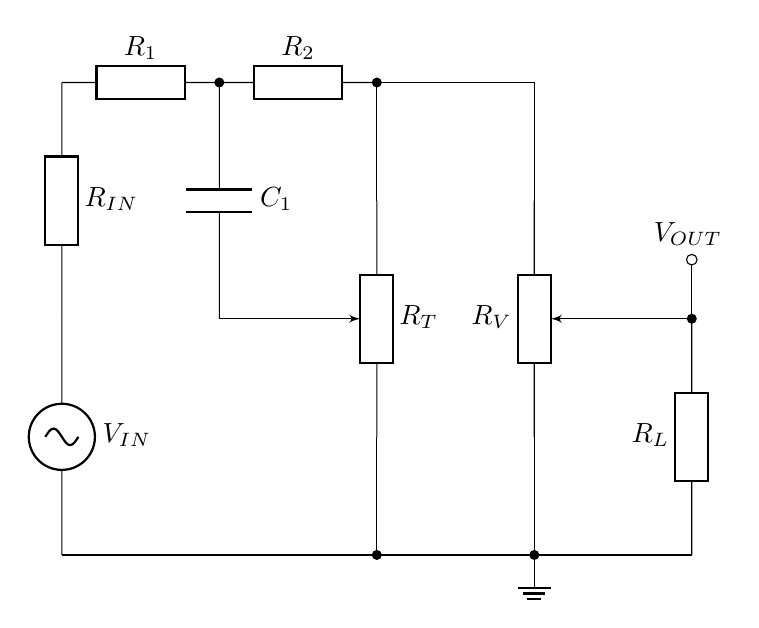
\begin{tikzpicture}
	% Instances/Symbols:
	\draw (1, 4) to[sinusoidal voltage source, l=$V_{IN}$] (1, 1);

	\draw (1, 7) to[european resistor, l=$R_{IN}$] (1, 4);	
	\draw (1, 7) to[european resistor, l=$R_1$] (3, 7);
	\draw (3, 7) to[european resistor, l=$R_2$] (5, 7);
	\draw (9, 4) to[european resistor, l_=$R_L$] (9, 1);

	\draw (3, 7) to[capacitor, l=$C_1$] (3, 4);

	\draw (5, 2.5) to[european potentiometer, l_=$R_T$] (5, 5.5);	
	\draw (7, 5.5) to[european potentiometer, l_=$R_V$] (7, 2.5);	

	% Lines:
	\draw (5, 5.5) -- (5, 7);
	\draw (5, 7) -| (7, 5.5);
	\draw (5, 1) -- (5, 2.5);
	\draw (3, 4) -- (4.5, 4);
	\draw (9, 4) -- (7.5, 4);
	\draw (1, 1) -- (9, 1);
	\draw (7, 2.5) -- (7, 1);
	\draw (9, 4) -- (9, 4.75);

	% Nodes:
	\node[ground] at (7, 1) {};
	\node[circ] at (3, 7) {};
	\node[circ] at (5, 7) {};
	\node[circ] at (5, 1) {};
	\node[circ] at (7, 1) {};
	\node[circ] at (9, 4) {};
	\node[ocirc, scale=1.2] at (9, 4.75) {};

	% Labels:
	\node[above=0.05cm of {8.95, 4.75}] {$V_{OUT}$};

\end{tikzpicture}
\end{document}